\label{PersistentHomology}
This chapter aims to provide an introduction to persistent homology\index{homology}\index{persistent homology\index{homology}}, demonstrating how it can be used to identify multiscale topological features\index{topological features} through the application of filtrations\index{filtrations} to complex data sets represented as point clouds\index{point clouds}. It discusses barcode\index{barcode} isomorphisms\index{isomorphisms} and persistence modules\index{modules}\index{persistence modules\index{modules}} that visualise and explain the stability of the detected features within a filtration\index{filtration} against perturbations of the data. 
The Stability Theorem\index{stability theorem} will not be discussed in this thesis \cite[Theorem 4.20]{chazal2016structure}, as it falls outside the scope of the subject under examination. The chapter concludes with a discussion of persistent chain complexes\index{chain complexes} and the cohomology\index{cohomology} of these structures, which contribute to a deeper understanding of the evolution of the topology\index{topology} of filtrations\index{filtrations} on point clouds\index{point clouds}.

\section{Filtrations of Complexes}
\label{FiltrationsofComplexes}
The following individual (co)homology\index{homology} groups are defined with coefficients in a fixed field, which we shall denote by $\F$, and form a graded module over the ring of polynomials in one variable $\F[t]$. Replacing the field with a ring leads to substantial problems, but most results still hold for principal ideal domains, see \cite[Theorem 2.1, \S 3.1]{zomorodian2004computing}. The first step is to define the cell complex, as every simplicial complex is a cell complex. In this section, we continue to examine the consequences of absolute and relative homology\index{homology} and cohomology\index{cohomology} groups for filtrations\index{filtrations} of cell complexes, such as the introduced simplicial complexes. In particular, we derive the theory in the context of filtered simplicial complexes upon sets of points, embedded into some metric space. While we can apply the entire theory to simplicial complexes and their (co)homology\index{homology}, cell complexes provide a much broader context and significantly simplify notation in many instances.

This yields a generalisation of the given situation.

\begin{definition}[\(d\)-cell]
A \(d\)-cell is a topological space that is homeomorphic to the open \(d\)-dimensional ball $\mathbb{B}^d = \{ x \in \mathbb{R}^d \; \vert \; \|x\| < 1 \}$, for any norm $\Vert \cdot \Vert$.
\end{definition}

\begin{example}\noindent
\begin{itemize}
    \item A $0$-cell is a single point, homeomorphic to \(\mathbb{B}^0 = \{ 0 \}\).
    \item A $1$-cell is an open line segment, homeomorphic to the open interval \((-1, 1)\).
    \item A $2$-cell is an open disk, homeomorphic to \(\mathbb{B}^2 = \{ (x, y) \; \vert \; x^2 + y^2 < 1 \}\).
    \item A $3$-cell is an open ball, homeomorphic to \(\mathbb{B}^3 = \{ (x, y, z) \; \vert \; x^2 + y^2 + z^2 < 1 \}\).
\end{itemize}
\end{example}

\begin{definition}[Cell complex]
A cell complex is a Hausdorff topological space \(X\) together with a filtration\index{filtration}
\begin{align}
\mathcal{X}: \quad \emptyset \subset X^0 \subset X^1 \subset X^2 \subset \cdots \subseteq X = \bigcup_{k=0}^{\infty} X^k =: X^\infty
\end{align}
such that:
\begin{enumerate}
    \item \(X^0\) is a discrete set of points.
    \item For each \(k \geq 1\), \(X^k\) is obtained from \(X^{k-1}\) by attaching a collection of \(k\)-cells \(\{\sigma^{(k)}_i\}_{i \in I_k}\) via continuous maps \(\varphi_i : S^{k-1} \to X^{k-1}\) from the $(k-1)$-sphere, where \(I_k\) is an indexing set for the \(k\)-cells of the cell complex. This set may be finite or infinite, depending on the number of \(k\)-cells. Each \(i \in I_k\) is an index that uniquely identifies a \(k\)-cell \(\sigma^{(k)}_i\) in the set of all \(k\)-cells of the complex. Specifically,
\begin{align}
    X^k = X^{k-1} \cup \bigcup_{i \in I_k} \sigma^{(k)}_i,
\end{align}
    where each \(\sigma^{(k)}_i \cong \mathbb{B}^k\) and \(\sigma^{(k)}_i \cap X^{k-1} = \varphi_i(S^{k-1})\).
    \item The topology\index{topology} on \(X\) is the weak topology\index{topology} with respect to the cells \(\{\sigma^{(k)}_i\}\).
\end{enumerate}
\end{definition}

\begin{remark}
A cell complex satisfies the following conditions:
\begin{itemize}
    \item The closure \(\overline{\sigma^{(m)}_i}\) intersects only finitely many cells \(\sigma^{(n)}_j\) for \(n \leq m, \text{and } n,m,i,j \in \mathbb{N}_0\).
    \item A set \(A \subseteq X\) is closed if and only if \(A \cap X^k\) is closed in \(X^k\) for all \(k \in \mathbb{N}_0\).
\end{itemize}
\end{remark}

\begin{proposition}
A simplicial complex is a cell complex.
\end{proposition}

\begin{proof}
Let \(K\) be a simplicial complex. We construct \(K\) as a cell complex by
\begin{align}
\mathcal{K}: \quad \emptyset \subset K^0 \subset K^1 \subset K^2 \subset \cdots \subset K = \bigcup_{k=0}^{\infty} K^k,
\end{align}
where \(K^k\) is the \(k\)-skeleton of \(K\). The $0$-skeleton \(K^0\) consists of the $0$-simplices, which form a discrete set. Assume \(K^{k-1}\) is constructed. To form \(K^k\), we attach each \(\natural\)-simplex \(\sigma^{(\natural)} \in K\) to \(K^{k-1}\) via a map \(\varphi_{\sigma^{(\natural)}} : \partial_{\natural} \sigma^{(\natural)} \to K^{k-1}\), where \(\partial_{\natural} \sigma^{(\natural)}\) is the boundary of \(\sigma^{(\natural)}\). Each \(\sigma^{(\natural)}\) is homeomorphic to an open \(\natural\)-ball \(\mathbb{B}^{\natural}\), and \(\partial_{\natural} \sigma^{(\natural)}\) is homeomorphic to the \((\natural-1)\)-sphere \(S^{\natural-1}\). The topology\index{topology} on \(|\tilde{K}|\), the geometric realization of the vertex scheme of \(K\), is the weak topology\index{topology} with respect to the simplices, thereby satisfying the topology\index{topology} condition of a cell complex. The closure-finite condition is satisfied because the closure of each simplex intersects only finitely many simplices. The proof is completed by induction over $\natural, k$.
\end{proof}

We investigate the persistent topology\index{topology} of filtered topological spaces, focusing primarily on the prototypical example of a filtered cell complex $\mathcal{X}: \emptyset \subset X^{0} \subset X^{1} \subset X^{2} \subset \cdots \subseteq X = \bigcup_{k=1}^{\infty} X^{k} =: X^\infty$, where \(X^{0}\) starts with vertices \(\sigma^{(0)}_a\), $a \in I_0$ the index set of all $\natural$-simplices, and each subsequent complex \(X_{i}\) is constructed by adding cells to the previous complex $X^{k} := X^{k-1} \cup \{\sigma^{(\natural)}\}_{a \in I_{k}}$. Here, the indexing set is \(\{0, 1, 2, \ldots, k, \ldots\}\), denoting the filtration level, such that $a \in [k,k+1)$. The dimension of the simplex, denoted by $\natural$, can vary. Additionally, associated real values \(a_{i}\) are assigned to the indexing sets, satisfying \(a_{1} \leq a_{2} \leq \cdots \leq a_{k}\), to indicate for which parameter the particular simplex is created during some filtration process.

\begin{example}{\cite[\S 2.2, Example]{de2011dualities}}
	\label{filteredsphere}
	The following illustrative example is a cellular filtration\index{filtration} of the $2$-sphere, denoted by $\mathcal{S}^2$. This process constructs a cell complex and introduces an ordering among the cells to provide a useful framework for organising the cells. In this sequence, the cell $\sigma_{1}^{(0)}$ stands for the initial point. The set $S^{2}$ consists of two distinct points. In $S^{3}$ a path connecting $\sigma_{1}^{(0)}$ and $\sigma_{2}^{(0)}$ is added. $S^{4}$ extends this path with its reversal, from $\sigma_{2}^{(0)}$ to $\sigma_{1}^{(0)}$, thus distinguishing it from the path in $S^{3}$. Finally, $S^{5}$ and $S^{6}$ make a distinction between cells representing the upper and lower halves of the sphere, respectively.
	\begin{figure}[H]%
	    \centering
	    \subfloat{
		    	\begin{tikzpicture}
				  \coordinate (1) at (-1.3cm,0cm);
				  \coordinate (2) at (1.3cm,0cm);
				  \draw[color=white, looseness=0.5] (1) to[out=-60, in=240] (2);
				  \draw[color=white, dashed, looseness=0.5] (1) to[out=60, in=-240] (2);
				  \draw[color=white, looseness=1.6] (1) to[out=-90, in=270] (2);
				  \draw[color=white, looseness=1.6] (1) to[out=90, in=-270] (2);
				  \fill (canvas cs:x=-1.3cm,y=0cm) circle (2pt);
				  \fill[color=white] (canvas cs:x=1.3cm,y=0cm) circle (2pt);
				  \node at (-1.6,0.1) {$\sigma_1^{(0)}$};
				  \node at (1.67,0.1) {};
				  \node at (-1.5,1.2) {$S^1$};
				\end{tikzpicture}
	    }%
	    \hfill
	    \subfloat{
		        \begin{tikzpicture}
				  \coordinate (1) at (-1.3cm,0cm);
				  \coordinate (2) at (1.3cm,0cm);
				  \draw[color=white, looseness=0.5] (1) to[out=-60, in=240] (2);
				  \draw[color=white, dashed, looseness=0.5] (1) to[out=60, in=-240] (2);
				  \draw[color=white, looseness=1.6] (1) to[out=-90, in=270] (2);
				  \draw[color=white, looseness=1.6] (1) to[out=90, in=-270] (2);
				  \fill (canvas cs:x=-1.3cm,y=0cm) circle (2pt);
				  \fill (canvas cs:x=1.3cm,y=0cm) circle (2pt);
				  \node at (-1.6,0.1) {$\sigma_1^{(0)}$};
				  \node at (1.67,0.1) {$\sigma_2^{(0)}$};
				  \node at (-1.5,1.2) {$S^2$};
				\end{tikzpicture}
	    }%
	    \hfill
	    \subfloat{
		        \begin{tikzpicture}
				  \coordinate (1) at (-1.3cm,0cm);
				  \coordinate (2) at (1.3cm,0cm);
				  \draw[-latex, looseness=0.5] (1) to[out=-60, in=240] (2);
				  \draw[color=white, dashed, looseness=0.5] (1) to[out=60, in=-240] (2);
				  \draw[color=white, looseness=1.6] (1) to[out=-90, in=270] (2);
				  \draw[color=white, looseness=1.6] (1) to[out=90, in=-270] (2);
				  \fill (canvas cs:x=-1.3cm,y=0cm) circle (2pt);
				  \fill (canvas cs:x=1.3cm,y=0cm) circle (2pt);
				  \node at (-1.6,0.1) {$\sigma_1^{(0)}$};
				  \node at (1.67,0.1) {$\sigma_2^{(0)}$};
				  \node[fill=white] at (0,-0.4) {$\sigma_3^{(1)}$};
				  \node at (-1.5,1.2) {$S^3$};
				\end{tikzpicture}
	    }%
	    \newline
	    \subfloat{
		    	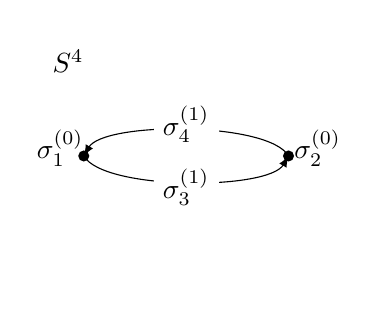
\begin{tikzpicture}
				  \coordinate (1) at (-1.3cm,0cm);
				  \coordinate (2) at (1.3cm,0cm);
				  \draw[-latex, looseness=0.5] (1) to[out=-60, in=240] (2);
				  \draw[latex-, looseness=0.5] (1) to[out=60, in=-240] (2);
				  \draw[color=white, looseness=1.6] (1) to[out=-90, in=270] (2);
				  \draw[color=white, looseness=1.6] (1) to[out=90, in=-270] (2);
				  \fill (canvas cs:x=-1.3cm,y=0cm) circle (2pt);
				  \fill (canvas cs:x=1.3cm,y=0cm) circle (2pt);
				  \node at (-1.6,0.1) {$\sigma_1^{(0)}$};
				  \node at (1.67,0.1) {$\sigma_2^{(0)}$};
				  \node[fill=white] at (0,-0.4) {$\sigma_3^{(1)}$};
				  \node[fill=white] at (0,0.4) {$\sigma_4^{(1)}$};
				  \node at (-1.5,1.2) {$S^4$};
				\end{tikzpicture}
	    }%
	    \hfill
	    \subfloat{
		        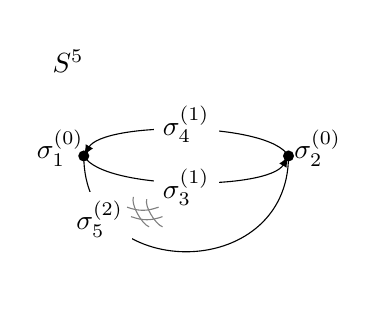
\begin{tikzpicture}
				  \coordinate (1) at (-1.3cm,0cm);
				  \coordinate (2) at (1.3cm,0cm);
				  \draw[-latex, looseness=0.5] (1) to[out=-60, in=240] (2);
				  \draw[latex-, looseness=0.5] (1) to[out=60, in=-240] (2);
				  \draw[looseness=1.6] (1) to[out=-90, in=270] (2);
				  \draw[color=white, looseness=1.6] (1) to[out=90, in=-270] (2);
				  \fill (canvas cs:x=-1.3cm,y=0cm) circle (2pt);
				  \fill (canvas cs:x=1.3cm,y=0cm) circle (2pt);
				  \node at (-1.6,0.1) {$\sigma_1^{(0)}$};
				  \node at (1.67,0.1) {$\sigma_2^{(0)}$};
				  \node[fill=white] at (0,-0.4) {$\sigma_3^{(1)}$};
				  \node[fill=white] at (0,0.4) {$\sigma_4^{(1)}$};
				  \node[fill=white] at (-1.1,-0.8) {$\sigma_5^{(2)}$};
				  \coordinate (a) at (-0.67cm,-0.52cm);
				  \coordinate (b) at (-0.47cm,-0.9cm);
				  \coordinate (c) at (-0.75cm,-0.65cm);
				  \coordinate (d) at (-0.35cm,-0.65cm);
				  \coordinate (c') at (-0.7cm,-0.77cm);
				  \coordinate (d') at (-0.3cm,-0.77cm);
				  \coordinate (a') at (-0.5cm,-0.55cm);
				  \coordinate (b') at (-0.3cm,-0.9cm);
				  \draw[color=gray, looseness=0.6] (a) to[out=250, in=160] (b);
				  \draw[color=gray, looseness=1] (c) to[out=-20, in=200] (d);
				  \draw[color=gray, looseness=1] (c') to[out=-20, in=200] (d');
				  \draw[color=gray, looseness=0.6] (a') to[out=250, in=160] (b');
				  \node at (-1.5,1.2) {$S^5$};
				\end{tikzpicture}
	    }%
	    \hfill
	    \subfloat{
		        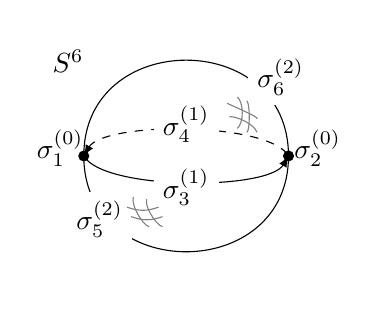
\begin{tikzpicture}
				  \coordinate (1) at (-1.3cm,0cm);
				  \coordinate (2) at (1.3cm,0cm);
				  \draw[-latex, looseness=0.5] (1) to[out=-60, in=240] (2);
				  \draw[latex-, dashed, looseness=0.5] (1) to[out=60, in=-240] (2);
				  \draw[looseness=1.6] (1) to[out=-90, in=270] (2);
				  \draw[looseness=1.6] (1) to[out=90, in=-270] (2);
				  \fill (canvas cs:x=-1.3cm,y=0cm) circle (2pt);
				  \fill (canvas cs:x=1.3cm,y=0cm) circle (2pt);
				  \node at (-1.6,0.1) {$\sigma_1^{(0)}$};
				  \node at (1.67,0.1) {$\sigma_2^{(0)}$};
				  \node[fill=white] at (0,-0.4) {$\sigma_3^{(1)}$};
				  \node[fill=white] at (0,0.4) {$\sigma_4^{(1)}$};
				  \node[fill=white] at (-1.1,-0.8) {$\sigma_5^{(2)}$};
				  \node[fill=white] at (1.2,1) {$\sigma_6^{(2)}$};
				  \coordinate (a) at (-0.67cm,-0.52cm);
				  \coordinate (b) at (-0.47cm,-0.9cm);
				  \coordinate (c) at (-0.75cm,-0.65cm);
				  \coordinate (d) at (-0.35cm,-0.65cm);
				  \coordinate (c') at (-0.7cm,-0.77cm);
				  \coordinate (d') at (-0.3cm,-0.77cm);
				  \coordinate (a') at (-0.5cm,-0.55cm);
				  \coordinate (b') at (-0.3cm,-0.9cm);
				  \draw[color=gray, looseness=0.6] (a) to[out=250, in=160] (b);
				  \draw[color=gray, looseness=1] (c) to[out=-20, in=200] (d);
				  \draw[color=gray, looseness=1] (c') to[out=-20, in=200] (d');
				  \draw[color=gray, looseness=0.6] (a') to[out=250, in=160] (b');
				  \coordinate (e) at (0.52cm,0.67cm);
				  \coordinate (f) at (0.9cm,0.47cm);
				  \coordinate (g) at (0.65cm,0.75cm);
				  \coordinate (h) at (0.65cm,0.35cm);
				  \coordinate (e') at (0.77cm,0.7cm);
				  \coordinate (f') at (0.77cm,0.3cm);
				  \coordinate (g') at (0.55cm,0.5cm);
				  \coordinate (h') at (0.9cm,0.3cm);
				  \draw[color=gray, looseness=0.3] (e) to[out=-30, in=20] (f);
				  \draw[color=gray, looseness=0.7] (g) to[out=-40, in=40] (h);
				  \draw[color=gray, looseness=0.7] (g') to[out=0, in=-250] (h');
				  \draw[color=gray, looseness=0.3] (e') to[out=-30, in=20] (f');
				  \node at (-1.5,1.2) {$S^6$};
				\end{tikzpicture}
	    }%
	\end{figure}

	\begin{itemize}
		\item[$\mathcal{S}^{2}:$] $\emptyset$
		\item[$\subset$] $S^{1} := \{\sigma_{1}^{(0)}\}$
		\item[$\subset$] $S^{2} := \{\sigma_{1}^{(0)}, \sigma_{2}^{(0)}\}$
		\item[$\subset$] $S^{3} := \{\sigma_{1}^{(0)}, \sigma_{2}^{(0)}, \sigma_{3}^{(1)} := (\sigma_{1}^{(0)}, \sigma_{2}^{(0)})\}$
		\item[$\subset$] $S^{4} := \{\sigma_{1}^{(0)}, \sigma_{2}^{(0)}, \sigma_{3}^{(1)}, \sigma_{4}^{(1)} := (\sigma_{2}^{(0)}, \sigma_{1}^{(0)})\}$
		\item[$\subset$] $S^{5} := \{\sigma_{1}^{(0)}, \sigma_{2}^{(0)}, \sigma_{3}^{(1)}, \sigma_{4}^{(1)}, \sigma_{5}^{(2)} := (\sigma_{3}^{(1)}, \sigma_{4}^{(1)})\}$
		\item[$\subset$] $S^{6} := \{\sigma_{1}^{(0)}, \sigma_{2}^{(0)}, \sigma_{3}^{(1)}, \sigma_{4}^{(1)}, \sigma_{5}^{(2)}, \sigma_{6}^{(2)} := (\sigma_{4}^{(1)}, \sigma_{3}^{(1)})\}.$
	\end{itemize}
\end{example}
\vspace{0.2cm}

\section{Persistence Modules}
\label{PersistenceModules}
Persistent homology\index{homology}\index{persistent homology\index{homology}} is derived by applying the homology\index{homology} functor to a filtration\index{filtration} of a topological space. This section will examine the concept of persistent modules\index{modules}, which serve to describe persistent homology\index{homology}\index{persistent homology\index{homology}} from an algebraic perspective. Similarly, as filtrations\index{filtrations} describe the evolution of a simplicial complex under a one-parameter or multi-parameter family, the persistence module describes the evolution of associated vector spaces. In the case of homology\index{homology} vector spaces or modules\index{modules}, the dimension or rank of the associated homomorphisms are the $k$-th Betti numbers, which indicates the number of $k$-dimensional holes of a topological space in intuitive terms.

\begin{definition}[Persistence module]{\cite[\S 1.1]{chazal2016structure}}
A real persistence module $\mathcal{C}(X)$ is a collection of vector spaces $\{V_i\}_{i \in I}$ over a partially ordered index set $(I,\leq)$ together with linear maps
\begin{align}
\phi_{r}^{s}: V_r \rightarrow V_s, \quad \forall r,s \in I: r \leq s,
\end{align}
such that $\phi_{r}^{t} = \phi^{t}_{s} \circ \phi_{r}^{s}$ and $\phi_{r}^r = \mathbb{I}_{V_r}$ for all $r \leq s \leq t$.
\end{definition}

We rephrase this definition in categorical language, which makes it easier for us to define the normal form of persistence modules\index{modules}\index{persistence modules\index{modules}}. Persistence modules\index{modules}\index{persistence modules\index{modules}} have a decomposition into interval modules\index{modules}, which cannot be further decomposed. On the other hand, an interval module is a persistence module that is indecomposable. Let $\operatorname{Vect}_\F$ be the category of finite dimensional vector spaces over $\F$. The reals are a partially ordered category $(\R, \leq)$. Consider the real persistence module:

\begin{definition}[Persistence module]{\cite[\S 1.3]{chazal2016structure}}
A persistence module is a functor $\mathcal{C}(X): (\R,\leq) \rightarrow \operatorname{Vect}_\F$. It is uniquely defined by a family $\{V_r\}_{r\in\R}$ of finite dimensional vector spaces over $\F$ together with morphisms $\phi_{r}^{s}: V_r \rightarrow V_s, r \leq s$, such that the following diagram commutes:
\begin{equation}
\begin{tikzcd}
V_r \arrow[d, "{\phi_{r}^{t}}" description] \arrow[r, "{\phi_{r}^{s}}" description] & V_s \\
V_t. \arrow[ru, "{\phi_{t}^{s}}" description]                                      &    
\end{tikzcd}
\end{equation}
\end{definition}

\begin{remark}
A morphism of persistence modules\index{modules}\index{persistence modules\index{modules}} is a natural transformation. This can be written as a morphism $f_r: V_r \rightarrow V'_r$, which is compatible with the maps $\phi_{r}^{s}$. This defines the category $\mathrm{Pers}$ of persistence modules\index{modules}\index{persistence modules\index{modules}}.
\end{remark}

The category of persistence modules\index{modules}\index{persistence modules\index{modules}} is abelian. A notable consequence of the aforementioned results is that a part of the constructions for persistence modules\index{modules}\index{persistence modules\index{modules}} remain valid when the category of finite-dimensional vector spaces over a field is replaced by another abelian category. This includes, for instance, (in)finite dimensional vector spaces over other fields. It is also possible to consider persistence modules\index{modules}\index{persistence modules\index{modules}} over cochain complexes in place of vector spaces.

In the following, we will make a number of simplifying assumptions:

\begin{assume}\noindent
\begin{enumerate}
	\item For all $r \in \R\backslash S$, where $S$ is a finite subset, there exists a neighbourhood $U_r$ of $r$ such that the map $\phi_u^{u'}$ is an isomorphism for all $u \leq u'$ in $U_r$.
	\item $V_u = 0$ for $u$ sufficiently small.
	\item For all $t \in \R$ and for all $s \leq t$ with $t-s$ sufficiently small, the mapping $\phi_s^t$ is an isomorphism.
\end{enumerate}
\end{assume}

The assumptions 1, 2 are referred to as finite type conditions. Assumption 1 implies that there is a finite number of 'jumps', while we have that $V_u = V_\infty$ for $u$ large enough. Assumption 3 is called semi-continuity and can be visualised by the following indecomposable interval modules\index{modules}:

\begin{definition}[Interval module]
Let $I$ be an interval of the form $(a,b]$ or $(a,\infty)$ with $-\infty < a < b \leq \infty$. We define an interval module $\mathbb{F}(I)$ over a field $\mathbb{F}$ as follows:
\begin{align}
	\mathbb{F}(I)_t = 
	\begin{cases}
		\mathbb{F}, & \text{if} \; t \in I, \\
		0, & \text{otherwise}.
	\end{cases}
\end{align}
The structure maps $f_{s}^t: \mathbb{F}(I)_s \to \mathbb{F}(I)_t$ for $s \leq t$ are defined as:
\begin{align}
	f_{s}^t = 
	\begin{cases}
		\mathrm{id}_{\mathbb{F}}, & \text{if } s, t \in I, \\
		0, & \text{if } s \notin I \text{ or } t \notin I.
	\end{cases}
\end{align}
\end{definition}

\subsection{Decomposition of Persistence Modules}
The following theorem describes the decomposition of any persistence module:

\begin{theorem}[Decomposition]{\cite[\S 1.5]{chazal2016structure}}
\label{decompositionPersistenceModules}
Every persistence module $\mathcal{C}(X)$ over a field $\mathbb{F}$ is isomorphic to a direct sum of interval modules\index{modules}:
\begin{align}
	\mathcal{C}(X) \cong \bigoplus_{i=0}^{d} \mathbb{F}(I_i)^{m_i},
\end{align}
where $I_i \neq I_j$ for all $i \neq j$, and $m_i$ are multiplicities. This decomposition is unique up to isomorphism and permutation of the summands.
\end{theorem}

\begin{proof}
To establish the existence of such a decomposition, we define a functor from the category $\mathrm{Pers}$ of persistence modules\index{modules}\index{persistence modules\index{modules}} to the category of finitely generated graded modules\index{modules} over the polynomial ring $\mathbb{F}[t]$. For a persistence module $\mathcal{C}(X) = \{V_t, f_{s}^t\}_{s \leq t}$, we map $\mathcal{C}(X)$ to the graded $\mathbb{F}[t]$-module $M = \bigoplus_{t \in \mathbb{R}} V_t$, where the action of $t$ on $M$ is defined by $t \cdot (v_0, v_1, \ldots) := (0, f_{0,1}(v_0), f_{1,2}(v_1), \ldots)$. The conditions ensuring the persistence module structure (finite generation and compatible transition maps) imply that $M$ is finitely generated as an $\mathbb{F}[t]$-module. This functor is an equivalence of categories: the inverse functor takes a graded $\mathbb{F}[t]$-module and interprets the grading as a persistence parameter over $\mathbb{R}$. Since $\mathbb{F}[t]$ is a principal ideal domain (PID), we can apply the structure theorem for finitely generated modules\index{modules} over a PID \cite[\S 2.1]{zomorodian2004computing}, which yields:
\begin{align}
	M = \bigoplus_{t \in \mathbb{R}} V_t \cong \bigoplus_{i=0}^d T^{\alpha_i} \mathbb{F}[t] \oplus \bigoplus_j T^{\gamma_j} \mathbb{F}[t] / (t^{d_j}).
\end{align}
Here, \( T^{\alpha_i} \mathbb{F}[t] \) denotes the graded free module over \( \mathbb{F}[t] \) shifted by \( \alpha_i \), meaning \( (T^{\alpha_i} \mathbb{F}[t])_d = \mathbb{F}[t]_{d - \alpha_i} \). This corresponds to interval modules\index{modules} of the form \( (\alpha_i, \infty) \). Similarly, \( T^{\gamma_j} \mathbb{F}[t] / (t^{d_j}) \) represents a torsion module over \( \mathbb{F}[t] \) that is shifted by \( \gamma_j \), defined by \( (T^{\gamma_j} \mathbb{F}[t] / (t^{d_j}))_d = \mathbb{F}[t]_{d - \gamma_j} / (t^{d_j}) \). This corresponds to interval modules\index{modules} of the form \( (\gamma_j, \gamma_j + d_j] \). 

For uniqueness, consider the endomorphism ring $\text{End}(\mathbb{F}(I))$. We show that $\text{End}(\mathbb{F}(I)) \cong \mathbb{F}$. Any endomorphism $\phi: \mathbb{F}(I) \to \mathbb{F}(I)$ must respect the persistence module structure, meaning $\phi_t: \mathbb{F}(I)_t \to \mathbb{F}(I)_t$ must be a linear map. Since $\mathbb{F}(I)_t = \mathbb{F}$ for $t \in I$ and $0$ otherwise, $\phi_t$ must be multiplication by a scalar $\lambda_t \in \mathbb{F}$. The critical technical reason for this is that $\mathbb{F}(I)_t$ is a simple module (i.e., it has no non-trivial submodules) when $t \in I$. Furthermore, for the endomorphism to be compatible with the structure maps $f_{s}^t$, we must have $\lambda_s = \lambda_t$ for all $s, t \in I$, meaning $\phi$ acts as multiplication by a constant $\lambda \in \mathbb{F}$ uniformly across the entire interval $I$. Hence, $\text{End}(\mathbb{F}(I)) \cong \mathbb{F}$.

Now, suppose we have two decompositions:
\begin{align}
	\bigoplus_i \mathbb{F}(I_i) \cong \mathcal{C}(X) \cong \mathcal{C}'(X) \cong \bigoplus_j \mathbb{F}(J_j).
\end{align}
Consider the composition of morphisms:
\begin{align}
	f_{ij}: &\mathbb{F}(I_i) \hookrightarrow \mathcal{C}(X) \cong \mathcal{C}'(X) \twoheadrightarrow \mathbb{F}(J_j),\\
	g_{ij}: &\mathbb{F}(J_j) \hookrightarrow \mathcal{C}'(X) \cong \mathcal{C}(X) \twoheadrightarrow \mathbb{F}(I_i).
\end{align}
The equation $\sum_{i,j} g_{ij}f_{ij} = 1$ implies that at least one of the compositions $f_{ij}g_{ij} \neq 0$, yielding an isomorphism between $\mathbb{F}(I_i)$ and $\mathbb{F}(J_j)$ for some $i, j$. Since the interval modules\index{modules} are indecomposable and distinct intervals $I_i$ and $J_j$ cannot yield non-trivial morphisms between each other, this forces $I_i = J_j$ and $m_i = m_j$. 

By induction on the number of summands, we conclude that the multiplicities $m_i$ and the intervals $I_i$ in both decompositions must coincide.
\end{proof}

\begin{definition}[Barcode\index{barcode}]
The barcode\index{barcode} associated with a persistence module $\mathcal{C}(X)$ is a collection of tuples consisting of interval modules\index{modules} and their corresponding multiplicities, given by the decomposition in Theorem \ref{decompositionPersistenceModules}:
\begin{align}
	\mathcal{B}(\mathcal{C}(X)) := \{(I_i, m_i)\}_{i=0}^d.
\end{align}
Here, each $I_i$ is an interval, and $m_i$ is the multiplicity of the interval module $\mathbb{F}(I_i)$ in the decomposition of $\mathcal{C}(X)$.
\end{definition}

At this point, we can establish a connection to spectral theory. In particular, for real-valued filtrations\index{filtrations}, the spectrum of a persistence module $\mathcal{C}(X)$ can be represented by specific intervals arising from the decomposition of persistence modules\index{modules}\index{persistence modules\index{modules}}.

\begin{definition}[Spectrum]
A point $t \in \mathbb{R}$ is called a spectral point of a persistence module $\mathcal{C}(X)$ if, for every neighborhood $U_t$ of $t$, there exist $s < r$ in $U_t$ such that the map $f_{s}^t$ is not an isomorphism. The (finite) spectrum of $\mathcal{C}(X)$ is defined as:
\begin{align}
	\text{Spec}(\mathcal{C}(X)) := \{ \text{spectral points} \} \cup \{\infty\}.
\end{align}
\end{definition}

\newpage
\begin{remark}\noindent
\begin{itemize}
    \item For each interval $I = (a,b]$ or $(a,\infty)$, and for any two points $s < r$ within this interval, the corresponding structure map $f_{s}^r$ of the persistence module $\mathcal{C}(X)$ is an isomorphism. A point $t$ becomes a spectral point if, within any neighborhood $U_t$ around $t$, there exists a pair $(s, r)$ such that the map $f_{s}^r$ is not an isomorphism. This identifies a change in the module's behavior, such as the birth of a new feature or the death of an existing one.
    \item The barcode\index{barcode} $\mathcal{B}(\mathcal{C}(X))$ provides a visual and combinatorial representation of the intervals and their multiplicities. Each interval in the barcode\index{barcode} corresponds to a range of points $t$ on the real line where the persistence module maintains consistent behavior. A spectral point indicates a transition between these behaviors, which corresponds to the endpoints of intervals in the barcode\index{barcode}.
    \item The spectrum $\text{Spec}(\mathcal{C}(X))$ summarizes the critical values on the real line where the module's structure changes. This concept is similar to the spectrum in functional analysis, where one considers the set of scalars (like eigenvalues) that describe how a linear operator acts on a vector space.
    \item Since the persistence module $\mathcal{C}(X)$ is finitely generated, the set of intervals in its decomposition is finite. This implies that the set of spectral points, which correspond to transitions between intervals, is also finite. The inclusion of $\infty$ in $\text{Spec}(\mathcal{C}(X))$ represents the asymptotic behavior of $\mathcal{C}(X)$, capturing the intervals of the form $(a, \infty)$.
\end{itemize}
\end{remark}

\subsection{Persistent Homology on Complexes}
\label{PersistentHomologyonComplexes}
In the context of algebraic topology\index{topology}, applying the homology\index{homology} functor $H(-)$
to a finite filtration\index{filtration} of a topological space $\mathcal{X}$ yields a sequence of algebraic structures:
\begin{equation}
	H(\mathcal{X}): \quad H(X^0) \rightarrow H(X^{1}) \to H(X^{2}) \to \cdots
	\to H(X^{d}) \rightarrow H(X),
\end{equation}
where $H(-)$ generally represents either the $k$-th dimensional
homology\index{homology}, denoted by $H_{k}(-;\F)$, or the absolute homology\index{homology}, expressed as $H
_{\bullet}(-;\F)$. Here, this diagram characterizes a sequence of abelian
groups or finite-dimensional vector spaces, connected through linear maps, forming a persistence module. Persistence modules\index{modules}\index{persistence modules\index{modules}} are central to understanding how the features of a space evolve
over time. According to Theorem \ref{decompositionPersistenceModules}, they can be decomposed into interval modules\index{modules}. Each interval module is associated with an
ordered pair of integers $(p,q)$ where $0 \leq p \leq q \leq d$, within a finite
filtration\index{filtration}. These pairs $(p,q)$ signify topological features\index{topological features} that persist over an
index set $I := \{p, \ldots, q\}$, where $\inf\{I\} = p$ and $\sup\{I\} = q$. Conventionally,
these tuples are interpreted as half-open intervals $[a_{p}, a_{q+1})$, with $a_{d+1}
= \infty$ being a customary notation when the sequence extends beyond the largest
indexed space. The decomposition of a persistence module into its constituent interval modules\index{modules} is
represented in a persistence diagram or a barcode\index{barcode}. This barcode\index{barcode} is a multiset of ordered tuples $(p,q)$ or, alternatively, a multiset
of half-open intervals $[a_{p}, a_{q+1})$. This collection is formally expressed
through the forgetful functor $\mathrm{Pers}(-)$, called the persistence diagram:
\begin{align}
    \mathrm{Pers}(H_k(\mathcal{X};\F)) & = \{(p_{1},q_{1}), \ldots, (p_{m},q_{m})\}                    \\
                                           & \cong \{[a_{p_1}, a_{q_1+1}), \ldots, [a_{p_m}, a_{q_m+1})\}.
\end{align}
In practical applications, intervals where $a_{p} = a_{q+1}$ are usually omitted,
as they represent ephemeral topological features\index{topological features}.

\begin{example}{\cite[\S 2.3, Example]{de2011dualities}}
    We consider the topological subspaces $S^{1}$,
    $S^{3}$, $S^{5}$, all of which are contractible. Meanwhile,
    $S^{2}$, $S^{4}$, $S^{6}$ are homeomorphic to the $0$-sphere, $1$-sphere, and $2$-sphere,
    respectively. This structural distinction leads to four distinct intervals in
    the persistence diagram of the absolute homology\index{homology} of a sphere, specifically $\mathcal{S}^{2}$:
    \begin{align}
        \mathrm{Pers}(H_{\bullet}(\mathcal{S}^{2})) & = \{(1,6)_{0}, (2,2)_{0}, (4,4)_{1}, (6,6)_{2} \}             \nonumber\\
                                                    & \cong \{[1,\infty)_{0}, [2,3)_{0}, [4,5)_{1}, [6, \infty)_{2} \}.
    \end{align}
    Here, the subscript $k$ in $(p,q)_{k}$ or $[a_{p}, a_{q+1})_{k}$ denotes a topological
    feature in the $k$-dimensional homology\index{homology}.
\end{example}

\subsection{The Four Standard Persistence Modules}
\label{TheFourStandardPersistenceModules}
\begin{figure}[t!]
	\begin{align*}
		H_{\bullet}(\mathcal{X})             & : \quad H_{\bullet}(X^{0}) \rightarrow H_{\bullet}(X^{1}) \rightarrow \cdots \rightarrow H_{\bullet}(X^{d-1}) \rightarrow H_{\bullet}(X^{d}),             \\
		H^{\bullet}(\mathcal{X})             & : \quad H^{\bullet}(X^{0}) \leftarrow H^{\bullet}(X^{1}) \leftarrow \cdots \leftarrow H^{\bullet}(X^{d-1}) \leftarrow H^{\bullet}(X^{d}),                \\
		H_{\bullet}(X^{\infty}, \mathcal{X}) & : \quad H_{\bullet}(X^{d}) \rightarrow H_{\bullet}(X^{d},X^{0}) \rightarrow H_{\bullet}(X^{d},X^{1}) \rightarrow \cdots \rightarrow H_{\bullet}(X^{d},X^{d-1}), \\
		H^{\bullet}(X^{\infty}, \mathcal{X}) & : \quad H^{\bullet}(X^{d}) \leftarrow H^{\bullet}(X^{d},X^{0}) \leftarrow H^{\bullet}(X^{d},X^{1}) \leftarrow \cdots \leftarrow H^{\bullet}(X^{d}, X^{d-1}).
	\end{align*}
	\caption{The four standard persistence modules are from top to bottom: persistent absolute homology, persistent absolute cohomology, persistent relative homology and persistent relative cohomology. The $(\bullet)$ indicates the direct sum of (co)homology over dimension, in other words the absolute (co)homology. We can also write $H^{\bullet}(X^{d}, \mathcal{X}), H_{\bullet}(X^{d}, \mathcal{X})$ or $H^{\bullet}(X, \mathcal{X}), H_{\bullet}(X, \mathcal{X})$ instead of $H^{\bullet}(X^{\infty}, \mathcal{X}), H_{\bullet}(X^{\infty}, \mathcal{X})$, as the $k$-th (co)homology groups for $k > d$ become trivial.}
\end{figure}
The standard module of absolute persistent homology\index{homology}\index{persistent homology\index{homology}}, $H_{\bullet}(\mathcal{X})$, illustrates how the absolute homology\index{homology} groups
$H_{\bullet}(X^{i})$ relate to each other as the index $i$ changes. Similar observations
can be made by considering the absolute cohomology\index{cohomology} groups $H^{\bullet}(X^{i})$,
the relative homology\index{homology} groups $H_{\bullet}(X^{d}, X^{i})$, and the relative cohomology\index{cohomology}
groups $H^{\bullet}(X^{d}, X^{i})$ \cite[\S 2.4]{de2011dualities}. The persistence diagram for absolute cohomology\index{cohomology} is represented as a multiset of integer
pairs $(p,q)$, where $0 \leq p \leq q \leq d$ for a finite filtration\index{filtration}. For relative
homology\index{homology} and cohomology\index{cohomology}, the persistence diagram consists of a multiset of
tuples $(p,q)$ where $0 \leq p \leq q \leq d-1$ for a finite filtration\index{filtration}. In each
case, we interpret $(p,q)$ as a half-open interval $[a_{p}, a_{q+1})$ with the
convention that $a_{0} = -\infty$ and $a_{d+1} = \infty$.

\begin{example}{\cite[\S 2.4, Example]{de2011dualities}}
	For $\mathcal{S}^{2}$ we yield
	\begin{align}
		\mathrm{Pers}(H_{\bullet}(S^{6},\mathcal{S}^{2})) & = \{(0,0)_{0}, (2,2)_{1}, (4,4)_{2}, (0,5)_{2}\}               \\
		                                                  & \cong \{[-\infty, 1)_{0}, [2,3)_{1}, [4,5)_{2}, [-\infty,6)_{3}\}.
	\end{align}
	At index $2$ there is a nontrivial element of $H_{1}(S^{6},S^{2})$ represented
	by any arc connecting the two points of $S^{2}$ --
	the homology\index{homology} class is $[\sigma_{3}] = [\sigma_{4}]$. This class vanishes in $H_{1}(S^{6},S^{3})$, thus we yield the interval $[2,3)$.
\end{example}

\section{Persistent (Co)homology}
\label{Persistent(Co)homology}
Inverse problems primarily involve inferring geometric shapes from measurements like
path integrals. Classical methods such as Fourier transforms provide extensive
information but struggle with nonlinearity and ill-posed conditions, requiring substantial
regularisation. Topology\index{topology}, particularly through persistent homology\index{homology}\index{persistent homology\index{homology}}, offers
alternative methods for deducing topological rather than geometric information. This
approach is especially useful in high-dimensional, discrete sets of points, exemplified
in the finite case by geological sonar to detect subterranean features based on density
variations \cite[\S 1]{de2011dualities}. Persistent homology\index{homology}\index{persistent homology\index{homology}} identifies
topological features\index{topological features} represented as intervals in a barcode\index{barcode} or persistence
diagram, crucial for understanding the presence and persistence of features such
as holes or voids in topological spaces. This method is statistically robust and
can provide both qualitative and quantitative insights into point sets, which we
suspect to lie on some compact topological object \cite{chazal2014persistence,chazal2009proximity}. We follow the results
of de Silva, Morozov, and Vejdemo-Johansson for our explanations \cite[\S 1]{de2011dualities}. In particular, there are at least four naturally arising persistent objects that
can be extracted from a filtration\index{filtration} of any topological space.
They are
\begin{equation*}
	\text{persistent}
	\begin{Bmatrix}
		\text{absolute} \\
		\text{relative}
	\end{Bmatrix}
	\begin{Bmatrix}
		\text{homology\index{homology}}   \\
		\text{cohomology\index{cohomology}}
	\end{Bmatrix}.
\end{equation*}
We address the computation of barcodes for all four types of persistent
objects. We demonstrate that both absolute and relative (co)homologies yield identical
barcodes and that transitions between these states are facilitated by established
duality principles. The duality between homology\index{homology} and cohomology\index{cohomology} is akin to the
duality in vector spaces, whereas a global duality specific to persistent topology\index{topology}
allows for a unique interchange:
\begin{align*}
	\text{Absolute homology\index{homology}}   & \rightleftarrows \text{relative cohomology\index{cohomology}.} \\
	\text{Absolute cohomology\index{cohomology}} & \rightleftarrows \text{relative homology\index{homology}.}
\end{align*}
The main results suggest that a single calculation is sufficient
to compute all four persistent objects due to the commutative nature of the global
duality.

\subsection{Barcode Isomorphisms}
\label{BarcodeIsomorphisms}
We characterise the multisets for persistence modules\index{modules}\index{persistence modules\index{modules}} that are decomposable into
interval modules\index{modules}. The persistence diagram partitions into $\mathrm{Pers}_{0}$,
comprising finite intervals $[a, b)$ as per \cite[\S 2.3]{de2011dualities}, and $\mathrm{Pers}_{\infty}$, consisting of intervals $[a, \infty)$. This leads to the decomposition
$\mathrm{Pers}= \mathrm{Pers}_{0} \cup \mathrm{Pers}_{\infty}$.

In this chapter, we establish that persistent homology\index{homology}\index{persistent homology\index{homology}} and cohomology\index{cohomology} yield the
same intervals, or barcodes, for both absolute and relative (co-)homology\index{homology}
frameworks. This equivalence necessitates invoking the Universal Coefficients Theorem
from algebraic topology\index{topology}, which we will prove beforehand. The universal coefficient
theorem for cohomology\index{cohomology} elegantly ties together the cohomology\index{cohomology} of a space with coefficients
in any abelian group $G$ to the homology\index{homology} of the space with integer coefficients. Specifically, as notation for this proof, $H_{d}(X;\mathbb{Z})$ and
$H^{d}(X;\mathbb{Z})$ denote the $d$-th singular homology\index{homology} and cohomology\index{cohomology} groups
with coefficients in $\mathbb{Z}$, respectively. We further involve
$\operatorname{Hom}(A, G)$, denoting group homomorphisms from an abelian group $A$ to another
abelian group $G$, and $\operatorname{Ext}^{1}(A, G)$ \cite[\S 3.1, p.195]{hatcher2005algebraic}, which measures obstructions
in the splitting of a short exact sequence of abelian groups. Further, we use the
properties of derived functors \cite[\S 2.7]{Weibel1994}.

\begin{theorem}[Universal coefficients for cohomology\index{cohomology}]{\cite[Theorem 3.2]{hatcher2005algebraic}}
\label{UniversalCoefficientsforCohomology}
Let $X$ be a topological space and $G$ an abelian group. For any integer $d \geq 0$, there is a short exact sequence:
\begin{align}
0 \rightarrow &\operatorname{Ext}^{1}(H_{d-1}(X;\mathbb{Z}), G) \rightarrow H^{d}(X; G) \rightarrow \cdots \\
\cdots \rightarrow &\operatorname{Hom}(H_{d}(X;\mathbb{Z}), G) \rightarrow 0,
\end{align}
which splits, though not canonically.
\end{theorem}

\begin{proof}
Let $(\mathcal{C}(X),\partial)$ be the singular chain complex of a topological space $X$ with integer coefficients. The homology\index{homology} groups $H_{d}(X; \mathbb{Z})$ are defined as:
\begin{align}
H_{d}(X; \mathbb{Z}) := \ker(\partial_{d}) / \operatorname{im}(\partial_{d+1}),
\end{align}
where $\partial_{d}$ are the boundary maps in $\mathcal{C}(X)$. The chain group $C_{d}(X)$ consists of formal sums of singular $d$-simplices in $X$ with integer coefficients. The boundary maps $\partial_{d}: C_{d}(X) \rightarrow C_{d-1}(X)$ are defined by
\begin{align}
\partial_{d}(\tilde{\sigma}^{(d)}) = \sum_{i=0}^{d}(-1)^{i} \tilde{\sigma}^{(d)}|_{[v_0, \ldots, \hat{v}_i, \ldots, v_d]},
\end{align}
where $\tilde{\sigma}^{(d)}: \tilde{\sigma}^{d} \rightarrow X$ is a singular simplex, and $\tilde{\sigma}|_{[v_0, \ldots, \hat{v}_i, \ldots, v_d]}$ denotes the restriction of $\tilde{\sigma}$ to the $i$-th face of the simplex, omitting the $i$-th vertex. The functor $\operatorname{Hom}(-, G)$ applied to $C_{d}(X)$ yields a group $\operatorname{Hom}(C_{d}(X), G)$, and the coboundary $\delta^{d}$ for the cochain complex $\operatorname{Hom}(\mathcal{C}^\flat(X), G)$ -- see Eq. \ref{cohomcomplex} -- is $\delta^{d}(f) = f \circ \partial_{d+1}$ for $f \in \operatorname{Hom}(C_{d+1}(X), G)$. This leads to the cohomology\index{cohomology groups} groups $H^{d}(X; G) := \ker(\delta^{d}) / \operatorname{im}(\delta^{d-1})$. We consider the projective resolution of $\mathcal{C}^\flat(X)$ to effectively apply the $\operatorname{Ext}^1$-functor. For an abelian group $A$, $\operatorname{Ext}^{1}(A, G) = R^{1} \operatorname{Hom}(A, G)$, where $R^{1}$ denotes the first right derived functor of $\operatorname{Hom}$ \cite[Vista 3.4.6, \S 3.5]{Weibel1994}. To show this equality, we begin by taking a projective resolution of $A$ \cite[Definition 2.2.4]{Weibel1994}: $\cdots \to P_{2} \to P_{1} \to P_{0} \to A \to 0$, where each $P_{i}$ is a projective abelian group. Then we can apply the functor $\operatorname{Hom}(-, G)$ to the projective resolution:
\begin{align}
0 \to \operatorname{Hom}(P_{0}, G) \to \operatorname{Hom}(P_{1}, G) \to \operatorname{Hom}(P_{2}, G) \to \cdots.
\end{align}
This sequence is exact on the left because $\operatorname{Hom}(-, G)$ is left exact and each $P_{i}$ is projective. The first right derived functor $R^{1}\operatorname{Hom}(A, G)$ is defined as the cohomology\index{cohomology} of this sequence at $P_{1}$:
\begin{align}
R^{1} \operatorname{Hom}(A, G) = \frac{\ker(\operatorname{Hom}(P_{1}, G) \to \operatorname{Hom}(P_{2}, G))}{\operatorname{im}(\operatorname{Hom}(P_{0}, G) \to \operatorname{Hom}(P_{1}, G))}.
\end{align}
The group $\operatorname{Ext}^{1}(A, G)$ classifies extensions of $A$ by $G$, equivalent to the kernel / image calculation in the cohomology\index{cohomology} of the $\operatorname{Hom}$-sequence $R^{1} \operatorname{Hom}(A, G)$. Given $H_{d}(X; \mathbb{Z})$, consider the short exact sequence obtained from the projective resolution of $\mathbb{Z}$: $0 \rightarrow \mathbb{Z} \rightarrow F \rightarrow H_{d}(X; \mathbb{Z}) \rightarrow 0$, where $F$ is free. Applying $\operatorname{Hom}(-, G)$ gives
\begin{align}
0 \rightarrow &\operatorname{Hom}(H_{d}(X; \mathbb{Z}), G) \rightarrow \operatorname{Hom}(F, G) \rightarrow \cdots \nonumber\\
\cdots \rightarrow &\operatorname{Hom}(\mathbb{Z}, G) \rightarrow \operatorname{Ext}^{1}(H_{d}(X; \mathbb{Z}), G) \rightarrow 0.
\end{align}
We apply $\operatorname{Ext}^{1}$, which gives rise to the long exact sequence of $\operatorname{Ext}^1$-groups:
\begin{align}
0 \rightarrow &\operatorname{Hom}(H_{d}(X; \mathbb{Z}), G) \rightarrow H^{d}(X; G) \rightarrow \cdots \nonumber\\
\cdots \rightarrow &\operatorname{Ext}^{1}(H_{d-1}(X; \mathbb{Z}), G) \rightarrow 0.
\end{align}
Finally, we verify exactness and splitting. The term $\operatorname{Ext}^{1}(H_{d-1}(X; \mathbb{Z}), G)$ measures the non-trivial extensions of $G$ by $H_{d-1}(X; \mathbb{Z})$, which corresponds to the obstructions to lifting $H_{d-1}(X; \mathbb{Z})$ linearly over $G$. The term $\operatorname{Hom}(H_{d}(X; \mathbb{Z}), G)$ represents the group homomorphisms from $H_{d}(X; \mathbb{Z})$ to $G$, which naturally includes in $H^{d}(X; G)$. The sequence is exact at each stage by the properties of derived functors and their application to the singular chain complex \cite[Horseshoe Lemma 2.2.8]{Weibel1994}. The sequence ends with $0$ because $\operatorname{Ext}^{1}$ of a projective (or free) module vanishes, and $\mathbb{Z}$ is free. The sequence splits because the functor $\operatorname{Hom}(-, G)$ preserves products and coproducts. However, the way it splits is not canonical and depends on the choice of a splitting homomorphism, which is not unique.

In the generalization of the Universal Coefficient Theorem \ref{UniversalCoefficientsforCohomology} to the case of modules\index{modules} over a PID, the $\operatorname{Ext}^{1}$ terms vanish since $\F$ is a field, thus we obtain $H^{d}(X;\F) \cong \operatorname{Hom}(H_{d}(X;\F),\F)$ \cite[\S 3.3.1, p.198]{hatcher2005algebraic}.
\end{proof}

\begin{theorem}{\cite[Proposition 2.3]{de2011dualities}}
For all integers $d \geq 0$, it holds that:
\begin{align}
\mathrm{Pers}(H_{d}(\mathcal{X};\F)) &= \mathrm{Pers}(H^{d}(\mathcal{X};\F)), \\
\mathrm{Pers}(H_{d}((X^{\infty}, \mathcal{X});\F)) &= \mathrm{Pers}(H^{d}((X^{\infty}, \mathcal{X});\F)).
\end{align}
\end{theorem}

\begin{proof}
When considering coefficients in a field $\F$ rather than in a ring, the Universal Coefficient Theorem \ref{UniversalCoefficientsforCohomology} assures us of a natural isomorphism between the $d$-th cohomology\index{cohomology} group and the homomorphisms from the $d$-th homology\index{homology} group to the base field: $H^{d}(X; \F) \cong \operatorname{Hom}(H_{d}(X; \F), \F)$. Therefore, the associated maps
\begin{equation}
H_{d}(X^{i}; \F) \rightarrow H_{d}(X^{j}; \F) \quad \text{and} \quad H^{d}(X^{i}; \F) \leftarrow H^{d}(X^{j}; \F)
\end{equation}
are adjoint and hence possess the same rank. Since the persistence intervals over a field are uniquely determined by the dimension and rank of the homology\index{homology} vector spaces, it follows that this holds for both homology\index{homology} and cohomology\index{cohomology}. Consequently, they share the same barcode\index{barcode}.
\end{proof}

Consider a finite filtration\index{filtration} $X^{0} \subset X^{1} \subset X^{2} \subset \cdots \subset X^d \subseteq X^{\infty}$ of a topological space $X$. The homology\index{homology} groups $H_{k}(X^{d})$ for some fixed dimension $k$ serve as the initial terms for the relative homology\index{homology} groups $H_{k}(X^{\infty}, X)$. Since $H_{k}(X)$ is consistent with $H_{k}(X^{d})$ as $d$ approaches infinity, these sequences can be unified into a single sequence: $H_{k}(X) \to H_{k}(X^{\infty}, X)$. For this concatenated sequence, the indices are 
\begin{align}
\{0, 1, 2, \ldots, d = \bar{0}, \bar{1}, \bar{2}, \ldots, \overline{(d-1)}\},
\end{align}
using the barred numbers to indicate relative homology\index{homology} part of the sequence. This structure allows us to discuss the persistence diagram associated with this homological configuration. The persistence intervals in this diagram can generally be categorized into three types:
\begin{enumerate}
	\item $(p, q)$ where $0 \leq p \leq q < d$, denoted as $[p, q+1)$ or $[a_{p}, a_{q+1})$.
	\item $(\bar{p}, \bar{q})$ where $0 < p \leq q \leq d-1$, denoted as $[\bar{p}, \bar{q}+1)$ or $[a_{\bar{p}}, a_{\bar{q}+1})$.
	\item $(p, \bar{q})$ where $0 \leq p \leq d, 0 \leq q \leq d-1$, denoted as $[p, \bar{q}+1)$ or $[a_{p}, a_{\bar{q}+1})$.
\end{enumerate}

\begin{corollary}{\cite[Proposition 2.5]{de2011dualities}}
The barcode\index{barcode} $\mathrm{Pers}(H_{k}(\mathcal{X}) \rightarrow H_{k}(X^{\infty}, \mathcal{X}))$ comprises the following collections of intervals, which match the previously discussed types of intervals bijectively:
\begin{enumerate}
    \item An interval $[a, b)$ for every interval $[a, b)$ in $\mathrm{Pers}_{0}(H_{k}(\mathcal{X}))$.
    \item An interval $[\bar{a}, \bar{b})$ for every interval $[a, b)$ in $\mathrm{Pers}_{0}(H_{k-1}(\mathcal{X}))$.
    \item An interval $[a, \bar{a})$ for every interval $[a, \infty)$ in $\mathrm{Pers}_{\infty}(H_{k}(\mathcal{X}))$.
\end{enumerate}
\end{corollary}

\begin{proof}
	We begin by analyzing the first two types of intervals in the persistence diagram
	$\mathrm{Pers}(H_{k}(X) \to H_{k}(X^{\infty}, X))$. These intervals either do
	not intersect the intermediate term $H_{k}(X{d})$ or terminate before it. Consequently,
	they correspond precisely to the finite intervals in $\mathrm{Pers}(H_{k}(X))$
	and $\mathrm{Pers}(H_{k}(X^{\infty}, X))$, clarifying the first two cases. The
	correspondence $\mathrm{Pers}_{0}(H_{k}(X^{\infty}, X)) = \mathrm{Pers}_{0}(H_{k-1}(X))$
	helps in mapping these relationships.

	The third case requires examining intervals of the form $[a, \bar{b})$ and
	proving that they are invariably of the form $[a, \bar{a})$, which means that
	the paired intervals $[a,\infty)$ and $[-\infty,a)$ in $\mathrm{Pers}_{\infty}(
	H_{k}(\X))$ and $\mathrm{Pers}_{\infty}(H_{k}(X^{\infty}, \X))$ are restrictions
	of a single interval $[a,\bar{a})$ in the concatenated sequence \cite[Proof of Proposition 2.5]{de2011dualities}.
	To establish this, we compare the ascending filtration\index{filtration} defined by the images of
	$H_{k}(X^{i})$ in $H_{k}(X^{d})$ for $i = 0, 1, 2, \ldots, d-1$ (denoted as
	$\operatorname{im}(H_{k}(X^{i}) \to H_{k}(X^{d}))$) with the descending filtration\index{filtration} defined
	by the kernels of $H_{k}(X^{d})$ in $H_{k}(X^{\infty}, X)$ for $i = 0, 1, 2, \ldots
	, d-1$ (denoted as $\ker(H_{k}(X^{d}) \to H_{k}(X^{d}, X^{i}))$). This
	examination revolves around the fundamental properties of the homology\index{homology} groups
	in a filtration\index{filtration} setting. For each index $i$, the image and kernel correspond to the same subspace of $H_{k}
	(X^{d})$. This equivalence is guaranteed by the homology\index{homology} long exact sequence
	associated with the pair $(X^{d}, X^{i})$, which links the relative and absolute
	homology\index{homology} groups. Specifically, the exact sequence implies that any cycle in $\operatorname{im}
	(H_{k}(X^{i}) \to H_{k}(X^{d}))$ that becomes a boundary in $H_{k}(X^{d}, X^{i}
	)$ must vanish, thus equating the image and kernel. As a result, both
	filtrations\index{filtrations} align perfectly, establishing that the third type of interval indeed
	maps to self-closing intervals of the form $[a, \bar{a})$.
\end{proof}

\subsection{Persistent Chain Complexes}
Alternatively, following \cite[\S 2.6]{de2011dualities}, the standard persistence module
can be described via a filtered cell complex $\mathcal{X}:= \bigcup_{i=0}^{d}\bigcup_{a \in I_d} \sigma_a^{(\natural)}$, adding cells for each filtration step, so that the persistence module is the sequence
\[
	\mathcal{C}(X): \quad C_{0} \to C_{1} \to C_{2} \to \cdots \to C_{d},
\]
for a finite filtration\index{filtration}, where each $C_{k}^{i} := \langle \{\sigma^{(k)}_a\}_{a \in I_0}, \{\sigma^{(k)}_a\}_{a \in I_1}, \ldots, \{\sigma^{(k)}_a\}_{a \in I_i}
\rangle$ is a vector space (or an abelian group) over a field $\F$, generated by the $k$-simplizes $\sigma^{(k)}_a$ for $a \in I_0, I_1, \ldots, I_i$. The boundary operator
is defined by $\partial_{\natural} \sigma^{(k)}_{j} = \sum_{i<j}\lambda_{ij}\sigma^{(k-1)}_{i}$ for $\lambda
_{ij}\in \F$ for all $i, j \in \{0, 1, \ldots, d\}$. Then $\mathcal{C}(X) = \{C_{k},\partial_{k}\}_{k=0}^{d}$ is the chain complex of $X$, and $\mathcal{C}(\mathcal{X})$ represents the persistent version for $\mathcal{X}$. This leads to the definition
of the persistent absolute homology\index{homology} of $\mathcal{X}$ as
\[
	H_{\bullet}(\mathcal{X}) = H(\mathcal{C}(X), \partial): \quad \frac{\ker(\partial_{0})}{\text{im}(\partial_{1})}
	\to \frac{\ker(\partial_{1})}{\text{im}(\partial_{2})} \to \frac{\ker(\partial_{2})}{\text{im}(\partial_{3})}\to \cdots \to \frac{\ker(\partial_{d})}{\text{im}(\partial_{d+1})}
	.
\]

For the persistent absolute cohomology\index{cohomology} $H^{\bullet}(\mathcal{X})$, we define
\[
	\label{cohomcomplex}
	\mathcal{C}^{\flat}(X): \quad C^{\flat}_{1} \leftarrow C^{\flat}_{2} \leftarrow \cdots
	\leftarrow C^{\flat}_{d},
\]
where $C_{i}^{\flat} = \text{Hom}(C_{i}, \F) = \langle \{\sigma^{(\natural)\flat}_a\}_{a \in I_0}, \{\sigma^{(\natural)\flat}_a\}_{a \in I_1}, \ldots, \{\sigma^{(\natural)\flat}_a\}_{a \in I_i} \rangle$, with the elements $\{\sigma^{(\natural)\flat}_a\}_{a\in I_j}$ as the dual basis of $\{\sigma^{(\natural)}_a\}_{a \in I_j}$. The coboundary $\delta
= \partial^{\flat}$ is defined as the adjoint of $\partial$. Considering $(\mathcal{C}^{\flat}(X), \delta)$, its homology forms a module structure $H^{\bullet}(\mathcal{X}) = H(\mathcal{C}^{\flat}(X), \delta) = \ker(\delta) / \text{im}(\delta)$. This is a persistence module, with morphisms in the reverse direction.

\begin{example}{\cite[\S 2.6, Example]{de2011dualities}}
	For $\mathcal{S}^{2}$, the boundary operator is given by
	\begin{align}
		\label{matrix}
		\partial_0\sigma^{(0)}_{1} & = \partial_0\sigma^{(0)}_{2} = 0, \nonumber\\
		\partial_1\sigma_{3}^{(1)} & = \partial_1\sigma_{4}^{(1)} = \sigma_{1}^{(0)}-\sigma_{2}^{(0)}, \nonumber\\
		\partial_2\sigma_{5}^{(2)} & = \partial_2\sigma_{6}^{(2)} = \sigma_{3}^{(1)} - \sigma_{4}^{(1)}.
	\end{align}
	Similarly, the coboundary operator is given by
	\begin{align}
		\label{transposed}
		\delta^0\sigma_{1}^{(0)\flat} = -\delta^0\sigma_{2}^{(0)\flat} & = \sigma_{3}^{(1)\flat} + \sigma_{4}^{(1)\flat}, \nonumber\\
		\delta^1\sigma_{3}^{(1)\flat} = -\delta^1\sigma_{4}^{(1)\flat} & = \sigma_{5}^{(2)\flat} + \sigma_{6}^{(2)\flat}, \nonumber\\
		\delta^2\sigma_{5}^{(2)\flat} = \delta^2\sigma_{6}^{(2)\flat}  & = 0.
	\end{align}
\end{example}

The data in Eq. \ref{matrix} and in Eq. \ref{transposed} can be summarized in a matrix and its transposed, respectively. The relative homology\index{homology} and cohomology\index{cohomology} persistence modules\index{modules}\index{persistence modules\index{modules}} are then defined as the homology\index{homology} of the persistence modules\index{modules}\index{persistence modules\index{modules}}:
	\begin{align*}
		(C_{d}/\mathcal{C}(X)):         & \quad C_{d} \rightarrow (C_{d}/C_{0}) \to (C_{d}/C_{1}) \rightarrow (C_{d}/C_{2}) \rightarrow \cdots \rightarrow (C_{d}/C_{d-1}),                             \\
		(C_{d}/\mathcal{C}(X))^{\flat}: & \quad C_{d}^{\flat} \leftarrow (C_{d}/C_{0})^{\flat} \to C_{d}/C_{1})^{\flat} \leftarrow (C_{d}/C_{2})^{\flat} \leftarrow \cdots \leftarrow (C_{d}/C_{d-1})^{\flat}.
	\end{align*}
We note that the mappings $\rightarrow$ from $\mathcal{C}(X)$ and the mappings $\leftarrow$ from $(C_{d}/\mathcal{C}(X))^{\flat}$ are injective, while the mappings $\leftarrow$ from $\mathcal{C}^{\flat}(X)$ and the mappings $\rightarrow$ from $(C_{d}/\mathcal{C}(X))$ are surjective. Thus, absolute and relative cohomology\index{cohomology} are structurally similar but qualitatively different from absolute homology\index{homology} and relative homology\index{homology}.

\begin{figure}
\centering
\begin{tikzcd}
                                  & \vdots \arrow[d, "\partial_{k+2}"]                                   & \vdots \arrow[d, "\partial_{k+2}"]                               & \vdots \arrow[d, "\partial_{k+2}"]                                            & \vdots \arrow[d, "\partial_{k+2}"]                                   &        \\
\cdots \arrow[r, "f^{i-1}_{i-2, k+1}"] & C_{k+1}^{i-1} \arrow[r, "f^{i}_{i-1, k+1}"] \arrow[d, "\partial_{k+1}"] & C_{k+1}^{i} \arrow[r, "f^{i+1}_{i, k+1}"] \arrow[d, "\partial_{k+1}"] & C_{k+1}^{i+1} \arrow[r, "f^{i+2}_{i+1, k+1}", no head] \arrow[d, "\partial_{k+1}"] & C_{k+1}^{i+2} \arrow[d, "\partial_{k+1}"] \arrow[r, "f^{i+3}_{i+2, k+1}"] & \cdots \\
\cdots \arrow[r, "f^{i-1}_{i-2, k}"]   & C_{k}^{i-1} \arrow[d, "\partial_{k}"] \arrow[r, "f^{i}_{i-1, k}"]       & C_{k}^{i} \arrow[d, "\partial_{k}"] \arrow[r, "f^{i+1}_{i, k}"]       & C_{k}^{i+1} \arrow[d, "\partial_{k}"] \arrow[r, "f^{i+2}_{i+1, k}"]                & C_{k}^{i+2} \arrow[d, "\partial_{k}"] \arrow[r, "f^{i+3}_{i+2, k}"]       & \cdots \\
\cdots \arrow[r, "f^{i-1}_{i-2, k-1}"] & C_{k-1}^{i-1} \arrow[d, "\partial_{k-1}"] \arrow[r, "f^{i}_{i-1, k-1}"] & C_{k-1}^{i} \arrow[d, "\partial_{k-1}"] \arrow[r, "f^{i+1}_{i, k-1}"] & C_{k-1}^{i+1} \arrow[d, "\partial_{k-1}"] \arrow[r, "f^{i+2}_{i+1, k-1}"]          & C_{k-1}^{i+2} \arrow[d, "\partial_{k-1}"] \arrow[r, "f^{i+3}_{i+2, k-1}"] & \cdots \\
                                  & \vdots                                                               & \vdots                                                           & \vdots                                                                        & \vdots                                                               &       
\end{tikzcd}
\caption{A persistent chain complex, where moving to the right increases the filtration\index{filtration} index, while moving downwards decreases the dimension. The maps $f_{i,k}^{i+1}$ correspond to the structure map from the $i$-th to the $(i+1)$-st chain group over $\mathbb{Z}$ -- or vector space over $\F$ -- in filtration step $k$. The boundary operator is defined for the chain complex, restricting it for each element to the respective chain group.}
\end{figure}

\begin{theorem}[Partition of persistence modules]
	{\cite[Theorem 2.6]{de2011dualities}} \label{persistencepartition} Let $\mathcal{C}(X)$ be given and $\partial$ as above, then there
	exists a partition $\{0,1,2, \ldots, d\} = B^{\Join} \sqcup B \sqcup D$ with a bijective pairing $B \leftrightarrow D$, such that $b$ is paired with $d$ if and only if $[b,d) \in \operatorname{Pairs}(\mathcal{C}(X), \partial)$. Furthermore, there is a basis
	$\hat{\sigma}^{(\natural)}_{0}, \hat{\sigma}^{(\natural)}_{1}, \hat{\sigma}^{(\natural)}_{2}, \ldots, \hat{\sigma}^{(\natural)}_{d}$ of $C_{d}$ such
	that
	\begin{itemize}
		\item $C_{i} = \langle \hat{\sigma}^{(\natural)}_{0}, \hat{\sigma}^{(\natural)}_{1}, \ldots, \hat{\sigma}^{(\natural)}_{i} \rangle$ for
			each $i$.
		\item $\partial_{\natural}\hat{\sigma}^{(\natural)}_{b} = 0$ for all $b \in B^{\Join}$.
		\item $\partial_{\natural}\hat{\sigma}^{(\natural)}_{d} = \hat{\sigma}^{(\natural)}_{b}$, and thus
			$\partial_{\natural}\hat{\sigma}^{(\natural)}_{b} = 0$, for all $[b,d) \in \operatorname{Pairs}$.
	\end{itemize}
	It follows that the persistence diagram
	$\operatorname{Pers}(H(\mathcal{C}(X),\partial))$ consists of $[a_{b}, \infty)$ for
	$b \in B^{\Join}$ together with intervals $[a_{b},a_{d})$ for
	$[b,d) \in \operatorname{Pairs}$.
\end{theorem}

\begin{proof}
	Let $\mathcal{C}(X) = \{C_{i}\}_{i \in I}$ be a filtered chain complex associated with
	a topological space, structured over a field $\F$ for any finite index
	set $I$. The filtration\index{filtration} indices ${0, 1, 2, \ldots, d}$, where $d = \vert I \vert$,
	classify the stages at which elements are born or die in homology\index{homology}. The
	partition of $\{0, 1, 2, \ldots, d\}$ into $B^{\Join} \sqcup B \sqcup D$ is then constructed such that $B^{\Join}$ contains indices corresponding to elements that persist indefinitely, i.e., those for which $\partial_{\natural}\sigma^{(\natural)}_{i} = 0$ and $\sigma^{(\natural)}_{i}$ does not become a boundary at any higher index. $B$ and $D$ are paired bijectively, where each $b \in B$ (births) corresponds uniquely to an $d \in D$ (deaths), signifying the termination of the homological feature introduced at $d$. This pairing is determined through the matrix reduction of $\partial$, ensuring that every cycle born at stage $b$ becomes a boundary at stage $d$. We then construct a basis ${\hat{\sigma}^{(\natural)}_i}$ such that for each $i$, $\hat{\sigma}^{(\natural)}
	_{i}$ is a generator of $C_{i}$. Specifically, if $i \in B^{\Join}$, then
	$\partial_{\natural}\hat{\sigma}^{(\natural)}_{i} = 0$, indicating these elements are cycles that persist
	indefinitely. For pairs $[b, d) \in \operatorname{Pairs}(\mathcal{C}(X), \partial)$
	with $b \in B$ and $d \in D$, set $\partial_{\natural}\hat{\sigma}^{(\natural)}_{d} = \hat{\sigma}^{(\natural)}_{b}$
	and $\partial_{\natural}\hat{\sigma}_{b} = 0$, reflecting the fact that the cycle
	$\hat{\sigma}^{(\natural)}_{b}$ born at $b$ becomes a boundary at $d$ and thus ceases to
	contribute to homology\index{homology} past $d$. Hence, the persistence diagram $\operatorname{Pers}(H(\mathcal{C}(X), \partial))$ contains
	intervals $[a_{b}, \infty)$ for each $b \in B^{\Join}$, indicating persistent
	homological features and intervals $[a_{b}, a_{d})$ for each
	$[b, d) \in \operatorname{Pairs}$, describing features with finite lifespans,
	starting as a cycle at $b$ and terminating as a boundary at $d$.
\end{proof}

\begin{remark}{\cite[\S 2, p.516]{Edelsbrunner2000}}
In Theorem \ref{persistencepartition} the index sets can be reexpressed in the original language of positive and negative simplices proposed by Edelsbrunner et al. \cite[p.8]{de2011dualities}, where a $(\natural)$-simplex is called positive if it belongs to a $\natural$-cycle and negative if it doesn't, respectively:
\begin{itemize}
	\item $B$ identifies the positive simplices that remain unpaired,
	\item $B^{\Join}$ identifies the positive simplices that do become paired,
	\item $D$ identifies the negative simplices.
\end{itemize}
The simplices $\hat{\sigma}^{(\natural)}_{b}$ and $\hat{\sigma}^{(\natural)}_{d}$ are cycles characterized by
their leading terms $\sigma^{(\natural)}_{b}$ and $\sigma^{(\natural)}_{d}$ respectively, while the simplex
$\hat{\sigma}^{(\natural)}_{d}$ is a chain with leading term $\sigma^{(\natural)}_{d}$. This chain 'kills'
the homology\index{homology} class of its paired cycle $\hat{\sigma}^{(\natural)}_{b}$ through the boundary relation
$\partial_{\natural} \hat{\sigma}^{(\natural)}_{d} = \hat{\sigma}^{(\natural)}_{b}$.
\end{remark}

\begin{theorem}{\cite[Proposition 2.4]{de2011dualities}}
	For all integers $d \geq 0$, it holds that:
	\begin{align*}
		\mathrm{Pers}_0(H_{d}(\mathcal{X})) \cong \mathrm{Pers}_0(H_{d+1}(X^\infty, \mathcal{X})), \nonumber\\
		\mathrm{Pers}_\infty(H_{d}(X^{\infty}, \mathcal{X})) \cong \mathrm{Pers}_\infty(H_{d}(X^{\infty}, \mathcal{X})).
	\end{align*}
\end{theorem}

\begin{proof}{\textit{\cite[Proof of Proposition 2.4]{de2011dualities}}}
The decomposition $\{0,1,2,\ldots,d\} = B^\Join \sqcup B \sqcup D$ and the new basis $\hat{\sigma}^{(\natural)}_0, \hat{\sigma}^{(\natural)}_1, \ldots, \hat{\sigma}^{(\natural)}_d$ allow us to write the persistent chain complex $\mathcal{C}(X)$ as a direct sum of persistent chain complexes, such that
\begin{align}
	\mathcal{C}(X) &= \bigoplus_{b^\Join \in B^\Join} \mathcal{C}(X)_{b^\Join} \oplus \bigoplus_{[b,d) \in \operatorname{Pairs}} \mathcal{C}(X)_{bd} \nonumber\\
	&= \bigoplus_{b^\Join \in B^\Join} \langle \hat{\sigma}_{b^\Join} \rangle \oplus \bigoplus_{[b,d) \in \operatorname{Pairs}} \langle \hat{\sigma}_{b}, \hat{\sigma}_{d} \rangle.
\end{align}
The boundary operator is compatible with this decomposition, where $\partial$ is defined for each summand as the corresponding boundary operator of the chain complex. Therefore, we can compute the homology $H((C_d/\mathcal{C}(X)),\partial)$ separately for each summand. For summands of the form $\mathcal{C}(X)_{b^\Join}$, the persistence modules are constant over two phases, with indices in $\{0,\ldots,b^\Join - 1\}$ and $\{b^\Join, \ldots, d-1\}$. Thus,
\begin{align}
	((C_{b^{\Join}})_d/\mathcal{C}(X)_{b^\Join})&: \quad \langle \hat{\sigma}^{(\natural)}_{b^\Join}\rangle \rightarrow 0,\nonumber\\
	\ker(\partial_{\natural})&: \quad \langle \hat{\sigma}^{(\natural)}_{b^\Join}\rangle \rightarrow 0,\nonumber\\
	\operatorname{im}(\partial_{\natural})&: \quad 0 \rightarrow 0,\nonumber\\
	H := \ker(\partial_\natural) / \operatorname{im}(\partial_{\natural+1})&: \quad \langle \hat{\sigma}^{(\natural)}_{b^\Join}\rangle \rightarrow 0.
\end{align}
It follows that $H((C_{b^\Join})_d/\mathcal{C}(X)_{b^\Join})$ contributes an interval of the form $[-\infty, a_{b^\Join})$, generated by the equivalence class of $[\hat{\sigma}^{(\natural)}_{b^\Join}]$, and thus has the same homological dimension as $[a_{b^{\Join}}, \infty) \in \operatorname{Pers}(H(\mathcal{C}(X)))$. For summands of the type $\mathcal{C}(X)_{bd}$, the persistence modules can be divided into constants over three phases, with indices in the ranges $\{0,\ldots,b-1\},$ $\{b,\ldots,b^{\Join}-1\}$, and $\{b^\Join,\ldots, d-1\}$, or explicitly:
\begin{align}
((C_{bd})_d/\mathcal{C}(X)_{bd}) &: \quad \langle \hat{\sigma}^{(\natural)}_b, \hat{\sigma}^{(\natural)}_d \rangle \rightarrow \langle \hat{\sigma}^{(\natural)}_d \rangle \rightarrow 0,\nonumber\\
\ker(\partial_\natural) &: \quad \langle \hat{\sigma}^{(\natural)}_b \rangle \rightarrow \langle \hat{\sigma}^{(\natural)}_d \rangle \rightarrow 0, \nonumber\\
\operatorname{im}(\partial_\natural) &: \quad \langle \hat{\sigma}^{(\natural)}_b \rangle \rightarrow 0 \rightarrow 0,\nonumber\\
H := \ker{\partial_\natural} / \operatorname{im}(\partial_\natural+1) &: \quad 0 \rightarrow \langle \hat{\sigma}^{(\natural)}_b \rangle \rightarrow 0.
\end{align}
It follows that $H((C_{bd})_d/\mathcal{C}(X)_{bd})$ contributes a single interval of the form $[a_b,a_d)$, generated by the equivalence class $[\hat{\sigma}^{(\natural)}_b]$, and thus has one dimension more than $[a_b,a_d) \in \operatorname{Pers}(H(\mathcal{C}(X)))$, which is generated by $[\hat{\sigma}^{(\natural)}_d]$.
\end{proof}

\begin{remark}{\cite[Proposition 2.4]{de2011dualities}}
	In this case, we get an isomorphism of multisets. This is due to the identification
	of the intervals $[a,\infty) \leftrightarrow [-\infty, a)$ for $\mathrm{Pers}_{\infty}$.
	Thus, persistent homology\index{homology}\index{persistent homology\index{homology}} and relative homology\index{homology} barcodes carry the same information,
	with a dimension shift for the finite intervals.
\end{remark}

In this closing argument, we will prove the four statements in Morozov's paper that were left open \cite[\S 2.8]{de2011dualities}.

Consider a finite filtration\index{filtration} of a topological space $X_0 \subseteq X_1 \subseteq \cdots \subseteq X_d = X$, with chain complexes\index{chain complexes} \( \mathcal{C}(X_i) := \{C^i_k, \partial_k)_{k \in \mathbb{N}_0} \}\) over \( \mathbb{F} \). We regard $\mathcal{C}(X)$ as a free module over $\F[t]$ with $d$ generators $\sigma^{(\natural)}_0, \sigma^{(\natural)}_1, \ldots, \sigma^{(\natural)}_d$, where $\sigma^{(\natural)}_i$ has degree $i$. This means w.l.o.g. that we add only a single cell at a time for each step within the filtration. The associated chain complexes\index{chain complexes} \( \mathcal{C}(X_i) \) over \( \mathbb{F} \) have inclusions \( X_i \subseteq X_{i+1} \) that induce structure maps \( f_{i}^{i+1}: C(X_i) \to C(X_{i+1}) \). The boundary operator $\partial: \mathcal{C}(X) \rightarrow \mathcal{C}(X)$ is a homomorphism of graded modules\index{modules}. We define the pointwise dual as the dual to the ground field $\F$, such that
\begin{align}
\mathcal{C}^\dagger(X) &= \Hom_\F(\mathcal{C}(X),\F), \\
C^\dagger_d&: C_{-d} \rightarrow \F \; \text{is a linear map.}
\end{align}
Analogously, we define the global dual as dual to the polynomial ring $\F[t]$:
\begin{align}
\mathcal{C}^\circ(X) &= \Hom_{\F[t]}(\mathcal{C}(X),\F[t]), \\
C^\circ_d&: \mathcal{C}(X) \rightarrow \F[t] \; \text{graded module homomorphism of degree $d$.}
\end{align}
These are graded $\F[t]$ modules\index{modules} themselves. The operations $-^\circ$ and $-\dagger$ are contravariant functors, thus the boundary map on $\mathcal{C}(X)$ induces boundary maps on the two new modules\index{modules} \cite[\S 2.8]{de2011dualities}.

\begin{theorem}\noindent
\begin{enumerate}
\item \(H(\mathcal{C}(X), \partial) \; \widehat{=} \; \text{persistent absolute homology\index{homology} of } \mathcal{X}.\)
\item \(H(\mathcal{C}^\dagger(X), \partial^\dagger) \; \widehat{=} \; \text{persistent absolute cohomology\index{cohomology} of } \mathcal{X}.\)
\item \(H(\mathcal{C}^\circ(X), \partial^\circ) \; \widehat{=} \; \text{persistent relative cohomology\index{cohomology} of } \mathcal{X}.\)
\item \(H(\mathcal{C}^{\circ\dagger}(X), \partial^{\circ\dagger}) \; \widehat{=} \; \text{persistent relative homology\index{homology} of } \mathcal{X}.\)
\end{enumerate}
\end{theorem}

\begin{proof}\noindent
\begin{enumerate}
\item Let \( \mathcal{X} = \{ X_i \}_{i=0}^d \) be a filtration of a topological space \( X \), where \( X_0 \subseteq X_1 \subseteq \cdots \subseteq X_d = X \). The persistent homology of this filtration is given by the persistent homology groups $H_k(X_i \subseteq X_j) = \mathrm{im} \left( H_k(X_i) \to H_k(X_j) \right)$, where \( H_k(X_i) \) is the \( k \)-th homology group of \( X_i \), and the map is induced by the inclusion \( X_i \subseteq X_j \).

To describe this algebraically, let \( \mathcal{C}(X) \) be the free graded module over the polynomial ring \( \mathbb{F}[t] \), generated by the chain complexes \( C_k^i \) being \( k \)-chains of \( X_i \). The multiplication by \( t \) in \( \mathcal{C}(X) \) represents the inclusion maps \( X_i \subseteq X_{i+1} \), encoding the structure of the filtration $f_{i,k}^j: C_k^i \to C_k^j$.

The boundary operator \( \partial \) on \( \mathcal{C}(X) \) satisfies \( \partial^2 = 0 \), and acts as a graded map that commutes with multiplication by \( t \). For each generator \( \sigma^{(\natural)}_k \in C_k^i \), we have $\partial_\natural(\sigma^{(\natural)}_k) \in C_{k-1}^i$. Thus, \( \partial \) is well-defined and consistent across the filtration.

The homology of \( \mathcal{C}(X) \) with respect to \( \partial \) is computed as $H_k(\mathcal{C}(X), \partial) = \frac{\ker(\partial_k)}{\mathrm{im}(\partial_{k+1})}$, where \( \partial_k: C_k^i \to C_{k-1}^i \) is the boundary operator on \( k \)-chains.

Now, because \( t \) encodes the inclusions \( X_i \subseteq X_{i+1} \), the structure of \( \mathcal{C}(X) \) ensures that the homology \( H_k(\mathcal{C}(X), \partial) \) captures the persistent homology groups \( H_k(X_i \subseteq X_j) \). Specifically, we have $H(\mathcal{C}(X), \partial) \cong \bigoplus_{0 \leq i \leq j \leq d} H_k(X_i \subseteq X_j)$, which shows that the homology of the chain complex \( \mathcal{C}(X) \) is isomorphic to the persistent homology of the filtration \( \mathcal{X} \).
\item The persistent cohomology groups for a filtration \( \mathcal{X} = \{ X_i \}_{i=0}^d \) are defined as $H^k(X_i \subseteq X_j) = \mathrm{im} \left( H^k(X_j) \to H^k(X_i) \right)$, where \( H^k(X_i) \) denotes the \( k \)-th cohomology group of \( X_i \), and the map is induced by the inclusion \( X_i \subseteq X_j \).

To model this algebraically, we construct the dual chain complex \( \mathcal{C}^\dagger(X) \), defined as the dual module of \( \mathcal{C}(X) \), that is \( \mathcal{C}^\dagger(X) = \mathrm{Hom}_\F(\mathcal{C}, \mathbb{F}) \), where \( \mathcal{C}(X) \) is the chain complex associated with the filtration. If \( \mathcal{C}(X) \) is free with generators \( \sigma^{(\natural)}_0, \sigma^{(\natural)}_1, \ldots, \sigma^{(\natural)}_d \), corresponding to the basis elements of \( C_k^d \), then the dual basis $\sigma^{(\natural)^\dagger}_i \in \mathcal{C}^\dagger(X)$ is defined by \( \sigma^{(\natural)\dagger}_i(\sigma^{(\natural)}_j) = \delta_{ij} \), where \( \delta_{ij} \) is the Kronecker delta.

The boundary operator in the dual chain complex \( \mathcal{C}^\dagger(X) \), denoted \( \partial^\dagger \), is defined by $\partial^\dagger(\phi) = \phi \circ \partial$, for any \( \phi \in \mathcal{C}^\dagger(X) \). The operator \( \partial^\dagger \) is a graded map, increasing the degree by one, and satisfies \( (\partial^\dagger_{k+1})^2 = 0 \), similar to the original boundary operator \( \partial \).

The cohomology of the dual chain complex \( \mathcal{C}^\dagger(X) \) with respect to \( \partial^\dagger \) is computed as $H^k(\mathcal{C}^\dagger(X), \partial^\dagger) = \frac{\ker(\partial^\dagger_k)}{\mathrm{im}(\partial^\dagger_{k-1})}$, where \( \partial^\dagger_k: C_k^i \to C_{k+1}^{i+1} \) is the dual boundary operator acting on cochains. The structure of \( \mathcal{C}^\dagger \) reflects the algebraic properties of cochains under the action of inclusion maps \( f_{i,i+1}: X_i \to X_{i+1} \) in the dual setting.

Multiplication by \( t \) in \( \mathbb{F}[t] \), which reflects the inclusions in the filtration, also acts on the dual module \( \mathcal{C}^\dagger(X) \). This ensures that the persistent cohomology of the filtration \( \mathcal{X} \) is encoded in the cohomology of \( \mathcal{C}^\dagger(X) \).

Thus, the cohomology of the dual chain complex \( \mathcal{C}^\dagger(X) \) captures the persistent cohomology groups of the filtration, yielding the isomorphism $H^k(\mathcal{C}^\dagger(X), \partial^\dagger) \cong \bigoplus_{0 \leq i \leq j \leq d} H^k(X_i \subseteq X_j)$.
\item The persistent relative cohomology\index{cohomology} groups for this filtration\index{filtration} are defined as $H^k(X_i, X_j) = \operatorname{coker} \left( H^k(X_j) \to H^k(X_i) \right)$, where \( H^k(X_i) \) represents the \( k \)-th cohomology\index{cohomology} group of \( X_i \), and the map is induced by the inclusion \( X_i \subseteq X_j \). The dual boundary operator \( \partial^\circ: \mathcal{C}^\circ \to \mathcal{C}^\circ \) is $\partial^\circ(\psi) = \psi \circ \partial$, for any \( \psi \in \mathcal{C}^\circ \), ensuring that \( \partial^\circ \) is a graded module homomorphism of degree 1. This definition maintains \( (\partial^\circ)^2 = 0 \) because \( \partial^2 = 0 \) in the original chain complex. We compute \( H(\mathcal{C}^\circ, \partial^\circ) \): $H^k(\mathcal{C}^\circ, \partial^\circ) = \ker(\partial^\circ_k) / \ima(\partial^\circ_{k-1})$, where \( \partial^\circ_k: C^k(X_i) \to C^{k+1}(X_{i+1}) \). To establish the isomorphism with persistent relative cohomology\index{cohomology}, we note that the module \( \mathcal{C}^\circ \) encodes the algebraic structure of cochains with coefficients in \( \mathbb{F}[t] \), reflecting the filtration\index{filtration}'s inclusions in a dual setting. The action of \( t \) in \( \mathbb{F}[t] \) within \( \mathcal{C}^\circ \) represents the inclusion maps \( f_{i,i+1} \) from \( X_i \) to \( X_{i+1} \), while \( \partial^\circ \) acts compatibly as a graded map. Thus, \( H^k(\mathcal{C}^\circ, \partial^\circ) \) captures the persistent relative cohomology\index{cohomology} groups \( H^k(X_i, X_j) \) for all \( 0 \leq i \leq j \leq n \). Therefore, $H(\mathcal{C}^\circ, \partial^\circ) \cong \bigoplus_{0 \leq i \leq j \leq n} H^k(X_i, X_j)$.
\item We define the double dual complex \( \mathcal{C}^{\circ\dagger} = \Hom_\F(\mathcal{C}^\circ, \F) \), where \( \mathcal{C}^\circ = \Hom_{\mathbb{F}[t]}(\mathcal{C}, \mathbb{F}[t]) \) is the global dual complex. Thus, \( \mathcal{C}^{\circ\dagger} \) is the dual to \( \mathcal{C}^\circ \) over the field \( \mathbb{F} \), capturing cochains with coefficients in \( \mathbb{F} \). The dual boundary operator \( \partial^{\circ\dagger}: \mathcal{C}^{\circ\dagger} \to \mathcal{C}^{\circ\dagger} \) is defined by $\partial^{\circ\dagger}(\phi) = \phi \circ \partial^\circ$, for any \( \phi \in \mathcal{C}^{\circ\dagger} \). This definition ensures that \( (\partial^{\circ\dagger})^2 = 0 \) since \( (\partial^\circ)^2 = 0 \) in the dual complex \( \mathcal{C}^\circ \). We compute \( H(\mathcal{C}^{\circ\dagger}, \partial^{\circ\dagger}) \): $H_k(\mathcal{C}^{\circ\dagger}, \partial^{\circ\dagger}) = \ker(\partial^{\circ\dagger}_k) / \ima(\partial^{\circ\dagger}_{k+1})$, where \( \partial^{\circ\dagger}_k: C_k(X_i) \to C_{k-1}(X_{i+1}) \). To establish the isomorphism with persistent relative homology\index{homology}, we note that the module \( \mathcal{C}^{\circ\dagger} \) reflects the algebraic structure of chains in the dual-dual setting, with coefficients in \( \mathbb{F} \). The dual action captures the inverse of the inclusion maps \( f_{i,i+1} \) from \( X_i \) to \( X_{i+1} \), while \( \partial^{\circ\dagger} \) acts compatibly. Thus, \( H_k(\mathcal{C}^{\circ\dagger}, \partial^{\circ\dagger}) \) encodes the persistent relative homology\index{homology} groups \( H_k(X_i, X_j) \) for all \( 0 \leq i \leq j \leq n \). Finally, $H(\mathcal{C}^{\circ\dagger}, \partial^{\circ\dagger}) \cong \bigoplus_{0 \leq i \leq j \leq n} H_k(X_i, X_j)$.
\end{enumerate}
\end{proof}

\subsection{Cohomology of Chain Complexes}
Persistent relative cohomology\index{cohomology} is structurally similar to persistent absolute homology\index{homology} \cite[\S 2.7]{de2011dualities}. We adopt Morozov's notation for the reversed sequence:
\begin{align}
	(C_n / \mathcal{C}(X))^\sharp &: \quad C_n^\sharp \leftarrow (C_n / C_1)^\sharp \leftarrow \cdots \leftarrow (C_n / C_{n-1})^\sharp, \\
	\mathcal{C}^\perp &: \quad C_1^\perp \rightarrow C_2^\perp \rightarrow \cdots \rightarrow C_n^\perp,
\end{align}
where we set \( C_i^\perp := (C_n / C_{n-i})^\sharp \). It is already known that \( \sigma_1^\sharp, \ldots, \sigma_n^\sharp \) form a basis of \( C_n^\sharp \), dual to the generators \( \sigma_1, \ldots, \sigma_n \) of \( C_n \). We define \( \tau_i = \sigma^\sharp_{n+1-i} \), leading to
\begin{align}
	C_i^\perp = \langle \sigma_n^\sharp, \sigma_{n-1}^\sharp, \ldots, \sigma_{n+1-i}^\sharp \rangle = \langle \tau_1, \tau_2, \ldots, \tau_i \rangle
\end{align}
through elementary linear algebra, as can be seen in Example \ref{chaincomplexcohomology}.

\begin{proposition}
Let \( \partial \) be the boundary operator in homology\index{homology}. If \( \partial \sigma_j = \sum_{i < j} D_{ij} \sigma_i \), then the corresponding coboundary operator \( \delta \) in cohomology\index{cohomology} is given by $\delta \tau_j = \sum_{i < j} D_{ij}^\perp \tau_i$, where \( D_{ij}^\perp = D_{(n-j),(n-i)} \) is the transposed and reversed version of the matrix \( D_{ij} \). 
\end{proposition}

\begin{proof}
Recall the duality between homology\index{homology} and cohomology\index{cohomology}. The boundary operator \( \partial \) in homology\index{homology} is defined by its action on the basis elements \( \sigma_j \in C_n \) as $\partial \sigma_j = \sum_{i < j} D_{ij} \sigma_i$, where \( D_{ij} \) are the coefficients of the boundary map. The corresponding coboundary operator \( \delta \) in cohomology\index{cohomology} acts on the dual space \( C_n^\sharp \), which is spanned by the dual basis \( \{\sigma_1^\sharp, \ldots, \sigma_n^\sharp\} \), where \( \sigma_i^\sharp(\sigma_k) = \delta_{ik} \). Define \( \tau_i = \sigma^\sharp_{n+1-i} \), which reverses the index order in the dual space. The coboundary operator \( \delta \) is the adjoint of the boundary operator \( \partial \), meaning that for any \( \tau_j \in C_n^\sharp \), we have $\delta \tau_j (\sigma_k) = \tau_j(\partial \sigma_k)$. Substituting the expression for \( \partial \sigma_j \), we get $\partial \sigma_j = \sum_{i < j} D_{ij} \sigma_i$, and thus:
\begin{align}
\delta \tau_j (\sigma_k) = \tau_j\left( \sum_{i < j} D_{ij} \sigma_i \right) = \sum_{i < j} D_{ij} \tau_j(\sigma_i).
\end{align}
By definition of the dual basis, \( \tau_j(\sigma_i) = \delta_{n+1-j,i} \), which means the action of \( \delta \) on \( \tau_j \) depends on the corresponding entries of the boundary matrix \( D_{ij} \). The coboundary operator \( \delta \) is thus governed by the transposed and index-reversed matrix \( D^\perp \), where $D_{ij}^\perp = D_{(n-j),(n-i)}$. Therefore, the action of \( \delta \) on \( \tau_j \) is given by $\delta \tau_j = \sum_{i < j} D_{ij}^\perp \tau_i$. \end{proof}

\begin{remark}{\cite[\S 2.7]{de2011dualities}}
Due to the structural similarity of \( \mathcal{C}^\perp \) and \( \mathcal{C} \), persistent absolute cohomology\index{cohomology} is interpreted as 'relative persistent relative cohomology\index{cohomology}'.
\end{remark}

\begin{example}
\label{chaincomplexcohomology}
Consider the construction explicitly for \( C_3 \) with basis \( \{\sigma_1, \sigma_2, \sigma_3\} \). The dual basis vectors in \( C_3^\sharp \) are \( \{\sigma_1^\sharp, \sigma_2^\sharp, \sigma_3^\sharp\} \), and we set \( \tau_1 = \sigma_3^\sharp \), \( \tau_2 = \sigma_2^\sharp \), and \( \tau_3 = \sigma_1^\sharp \). For \( C_2^\perp \), we obtain:
\[
	C_2^\perp = \langle \sigma_3^\sharp, \sigma_2^\sharp \rangle = \langle \tau_1, \tau_2 \rangle.
\]
If the boundary map for \( \partial \sigma_3 \) is given by:
\[
	\partial \sigma_3 = D_{31} \sigma_1 + D_{32} \sigma_2,
\]
then the coboundary operator \( \delta \) acts on \( \tau_1 \) as:
\[
	\delta \tau_1 = D_{32}^\perp \tau_2 + D_{31}^\perp \tau_3,
\]
where \( D_{32}^\perp = D_{23} \) and \( D_{31}^\perp = D_{13} \) are the transposed entries.
\end{example}

\begin{proposition}{\cite[Proposition 2.8]{de2011dualities}}
The persistence module $(C_n^\perp/\mathcal{C}^\perp)$ is the reverse of $\mathcal{C}^\sharp$, and the respective coboundary maps agree.
\end{proposition}

\begin{proof}
Each submodule \( C_i^\perp \) is defined as the dual of the quotient \( C_n / C_{n-i} \), i.e., $C_i^\perp = (C_n / C_{n-i})^\sharp$. Thus, the persistence module \( (C_n^\perp / \mathcal{C}^\perp) \) is constructed by taking the quotient of \( C_n^\perp \) by \( \mathcal{C}^\perp \), which gives the reversed filtration\index{filtration}:
\begin{align}
C_n^\sharp \leftarrow (C_n / C_1)^\sharp \leftarrow \cdots \leftarrow (C_n / C_{n-1})^\sharp.
\end{align}
This is the filtration\index{filtration} of \( \mathcal{C}^\sharp \), but in reverse order. Therefore, the persistence module \( (C_n^\perp / \mathcal{C}^\perp) \) is the reverse of \( \mathcal{C}^\sharp \).

Consider the boundary operator \( \partial \) on the chain complex \( C_n \), given by $\partial \sigma_j = \sum_{i < j} D_{ij} \sigma_i$, where \( D_{ij} \) are the coefficients of the boundary operator. In the dual space \( C_n^\sharp \), the coboundary operator \( \delta \) acts on the dual basis elements \( \tau_j = \sigma^\sharp_{n+1-j} \). The coboundary map is induced by the transposed and reversed matrix of the boundary operator $\delta \tau_j = \sum_{i < j} D_{ij}^\perp \tau_i$, where \( D_{ij}^\perp = D_{(n-j),(n-i)} \), the transposed and index-reversed version of the boundary matrix \( D_{ij} \). Since the filtration\index{filtration} in \( (C_n^\perp / \mathcal{C}^\perp) \) corresponds to the reverse of \( \mathcal{C}^\sharp \), and the coboundary operators are induced by the same transposed matrix \( D^\perp \).
\end{proof}

\begin{corollary}{\cite[Proposition 2.10]{de2011dualities}}
Let \( \hat{\sigma}_1^\sharp, \ldots, \hat{\sigma}_n^\sharp \) be the dual of \( \hat{\sigma}_1, \ldots, \hat{\sigma}_n \), where $C_i = \langle \hat{\sigma}_1, \ldots, \hat{\sigma}_i \rangle$ for $1 \leq i \leq n$. Then \( \hat{\tau}_i = \hat{\sigma}_{n+1-i}^\sharp \) for all \( i \).
\end{corollary}

\begin{proof}
We use Theorem \ref{persistencepartition} and obtain a partition of indices \( \{1, 2, \ldots, n\} = R \sqcup S \sqcup T \) for \( \mathcal{C}^\perp \) and new generators \( \hat{\tau}_i \), where:
\begin{align}
\delta \hat{\tau}_i = 0 \quad \text{for } i \in R \sqcup T, \quad \delta \hat{\tau}_t = \hat{\tau}_s \quad \text{for pairs } (s,t) \in \text{Pairs}(\mathcal{C}^\perp, \delta).
\end{align}
Now, let \( \hat{\sigma}_1^\sharp, \ldots, \hat{\sigma}_n^\sharp \) denote the dual basis of \( \hat{\sigma}_1, \ldots, \hat{\sigma}_n \), such that:
\begin{align}
\hat{\sigma}_i^\sharp(\hat{\sigma}_j) = \delta_{ij} \quad \text{for all } i,j.
\end{align}
Since \( \mathcal{C}^\perp \) is the dual filtration\index{filtration} of \( \mathcal{C} \), we observe that the filtration\index{filtration} structure in \( \mathcal{C}^\perp \) is reversed. Specifically, the duality induces the relationship between the generators \( \hat{\tau}_i \) and the elements of the dual basis:
\begin{align}
\hat{\tau}_i = \hat{\sigma}_{n+1-i}^\sharp.
\end{align}
This indexing reversal arises naturally from the dual filtration\index{filtration} structure. The coboundary operator \( \delta \) respects this duality, so that for any pair \( (s,t) \in \text{Pairs}(\mathcal{C}^\perp, \delta) \), we have $\delta \hat{\tau}_t = \hat{\tau}_s$, preserving the dual pairing structure of the persistence module. Thus, for each \( i \), the relation \( \hat{\tau}_i = \hat{\sigma}_{n+1-i}^\sharp \) holds, completing the proof.
\end{proof}